\section{Durchführung}
\label{sec:Durchführung}
    \subsection{Untersuchung der Zeitabhängigkeit der Schwingungsamplituden}
        Mithilfe der Schaltung welche in \autoref{fig:schaltung1} zusehen ist wird die Zeitabhängigkeit der Schwingungsamplituden des LRC-Kreises gemessen.
        Ein Nadelimpulsgenerator erregt den Schwingkreis zu gedämpften Schwingungen. Mittels eines Tastkopfes, welcher die Schwingung zwischen Spule
        und Kondensator abnimmt, wird diese auf einen digitalen Oszillographen ausgegeben. Durch Verwendung des hochohmigen Tastkopfes ist der 
        Eingangswiderstand der Oszillographen vernachlässigbar klein. 
        Zu Beachten ist weiterhin den kleineren der beiden Festwiderstände zu verwenden.
        Mit der Cursor-Funktion des Oszillographen sind die Zusammenhänge von Zeitpunkt und Schwingungsamplituden zu messen und aufzunehmen.
        \begin{figure}
            \centering
            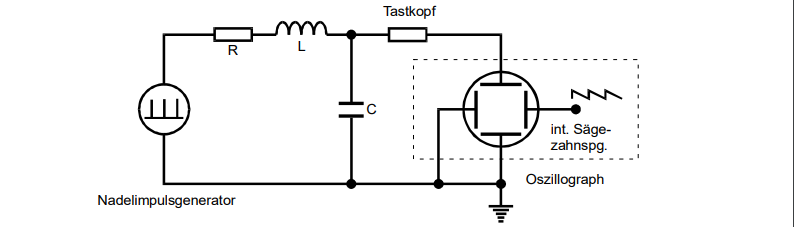
\includegraphics[width=\textwidth]{content/s1.png}
            \caption{Schaltung zur Bestimmung der Zeitabhängigkeit der Amplitude einer gedämpften Schwingung \cite[294]{V354}.}
            \label{fig:schaltung1}
        \end{figure} 
    \subsection{Bestimmung des Dämpfungswiderstand beim aperiodischen Grenzfall}    
        Bei diesem Versuchsteil wird wieder die Schaltung aus \autoref{fig:schaltung1} verwendet, mit dem Unterschied, dass statt dem Festwiderstand
        ein regelbarer Widerstand verwendet wird. Zunächst wird der Widerstand auf seinen Maximalwert gestellt, sodass ein reines Relaxationsverhalten
        auf dem Oszillographen zu sehen ist. Anschließend wird der Widerstand so lange heruntergeregelt, bis ein Überschwingen in der Kurve festzustellen ist.
        Der Widerstand ist dann so einzustellen, dass dieses Überschwingen gerade wieder verschwindet. Der eingestellte Widerstand wird aufgenommen.
    \subsection{Untersuchung der Frequenzabhängigkeit der Kondensatorspannung}
        Für diesen Versuchsteil wird die Schaltung wie in \autoref{fig:schaltung2} zu sehen aufgebaut, jedoch ohne die Nutzung des Zweitkanals des Oszillographen.
        Der Sinuswellengenerator gibt sinusförmige Wellen verschiedener Frequenzen auf den LRC-Kreis. Wie zuvor gibt ein Tastkopf die Schwingung
        wieder auf dem Oszillographen aus. Zuvor wird mithilfe des Tastkopfes die reine Erregerspannung gemessen und aufgenommen. Zu Beachten 
        ist weiterhin, dass in diesem Aufbau der größere der beiden Festwiderstände zu Benutzen ist. In Abhängigkeit der eingestellten Frequenzen
        werden nun die auf dem Oszillographen ausgegebenen Amplituden mittels der Cursor-Funktion ausgemessen und in Abhängigkeit der eingestellten
        Frequenz aufgenommen. Die einzustellenden Frequenzen sind im Bereich von $12$\,kHz bis $30$\,kHz und $44$\,kHz bis $62$\,kHz in $2$\,kHz Schritten zu wählen;
        im Bereich von $32$\,kHz bis $42$\,kHz sind $1$\,kHz Schritte zu wählen.
        \begin{figure}
            \centering
            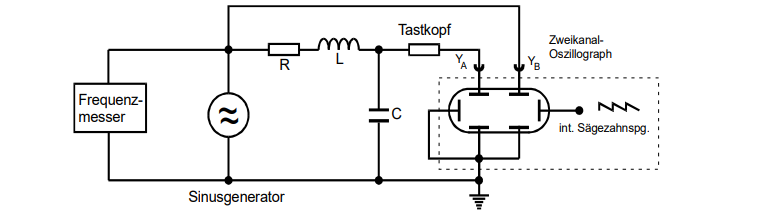
\includegraphics[width=\textwidth]{content/s2.png}
            \caption{Schaltung zur Bestimmung der Frequenzabhängigkeit der Amplitude der Kondensatorspannung, sowie der Phase zwischen Erreger - und Kondensatorspannung \cite[296]{V354}.}
            \label{fig:schaltung2}
        \end{figure} 
    \subsection{Untersuchung der Frequenzabhängigkeit der Phasendifferenz}
        Es wird wieder die Schaltung \autoref{fig:schaltung2} verwendet, diesmal jedoch unter Nutzung beider Oszillographeneingänge. Der Oszillograph
        zeigt nun zwei Kurven an. Der Abstand der Nulldurchgänge der beiden Kurven ist mittels der Oszillographen auszumessen und in 
        Abhängigkeit von der Frequenz zu notieren. Die einzustellenden Frequenzen sind die Selben, wie im Versuchsteil zuvor.    